\begin{figure}[H]
\centering
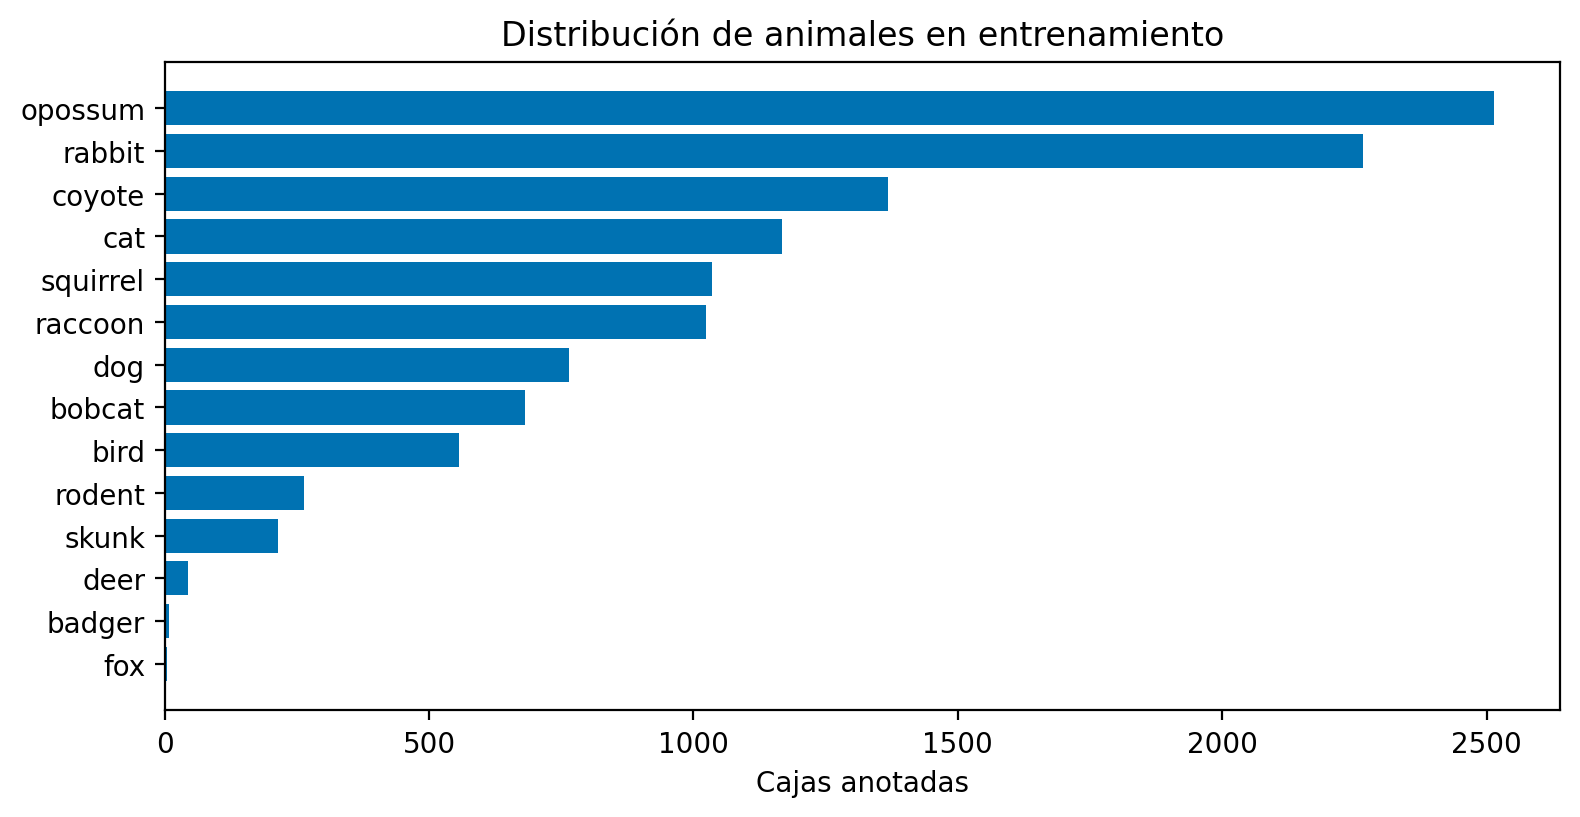
\includegraphics[width=0.74\linewidth]{figures/figure_0.png}
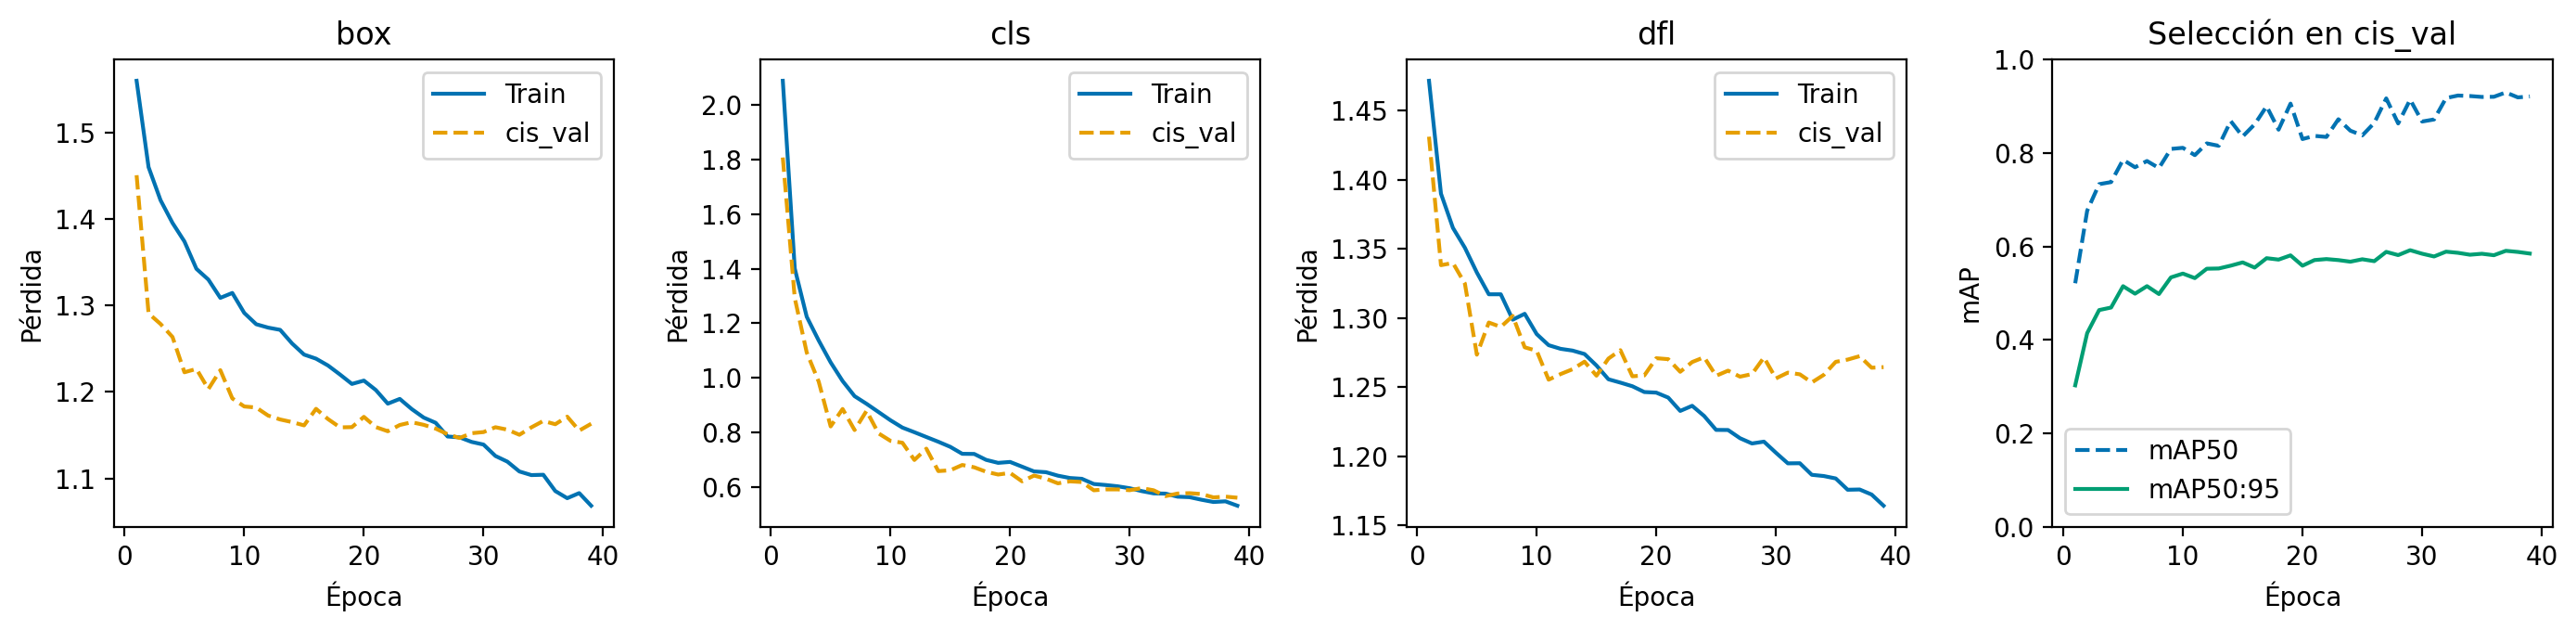
\includegraphics[width=\linewidth]{figures/figure_1.png}
\caption{Distribución de cajas de entrenamiento y evolución de pérdidas y mAP en cis\_val. El mejor checkpoint corresponde a la época 29; las curvas no utilizan los tests.}
\end{figure}

\begin{figure}[H]
\centering
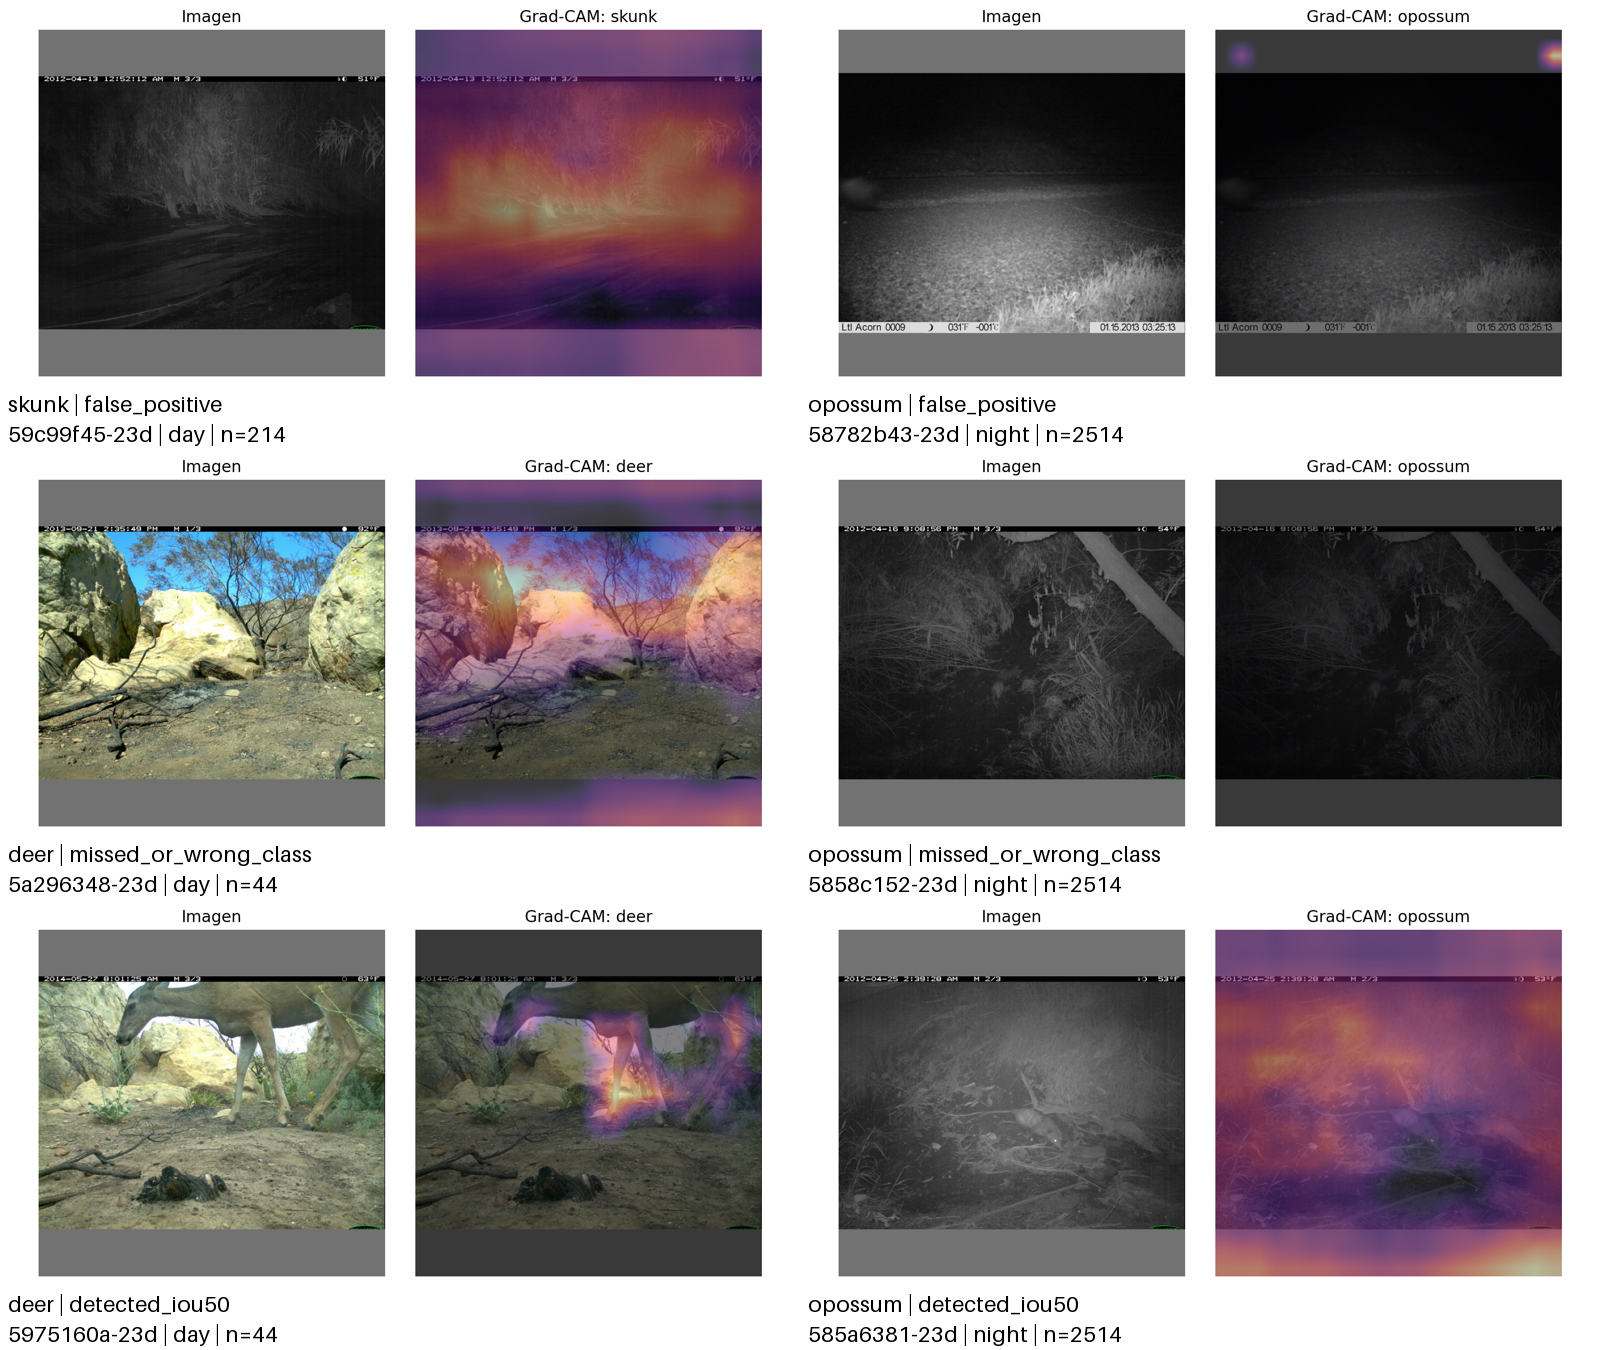
\includegraphics[width=\linewidth]{figures/figure_2.png}
\caption{Seis casos en cámaras conocidas. Se conserva el mapa plano de cis\_test\_3 como limitación del método; no se interpreta como evidencia de ausencia de atención. Los rótulos day/night son aproximaciones de metadatos.}
\end{figure}

\begin{figure}[H]
\centering
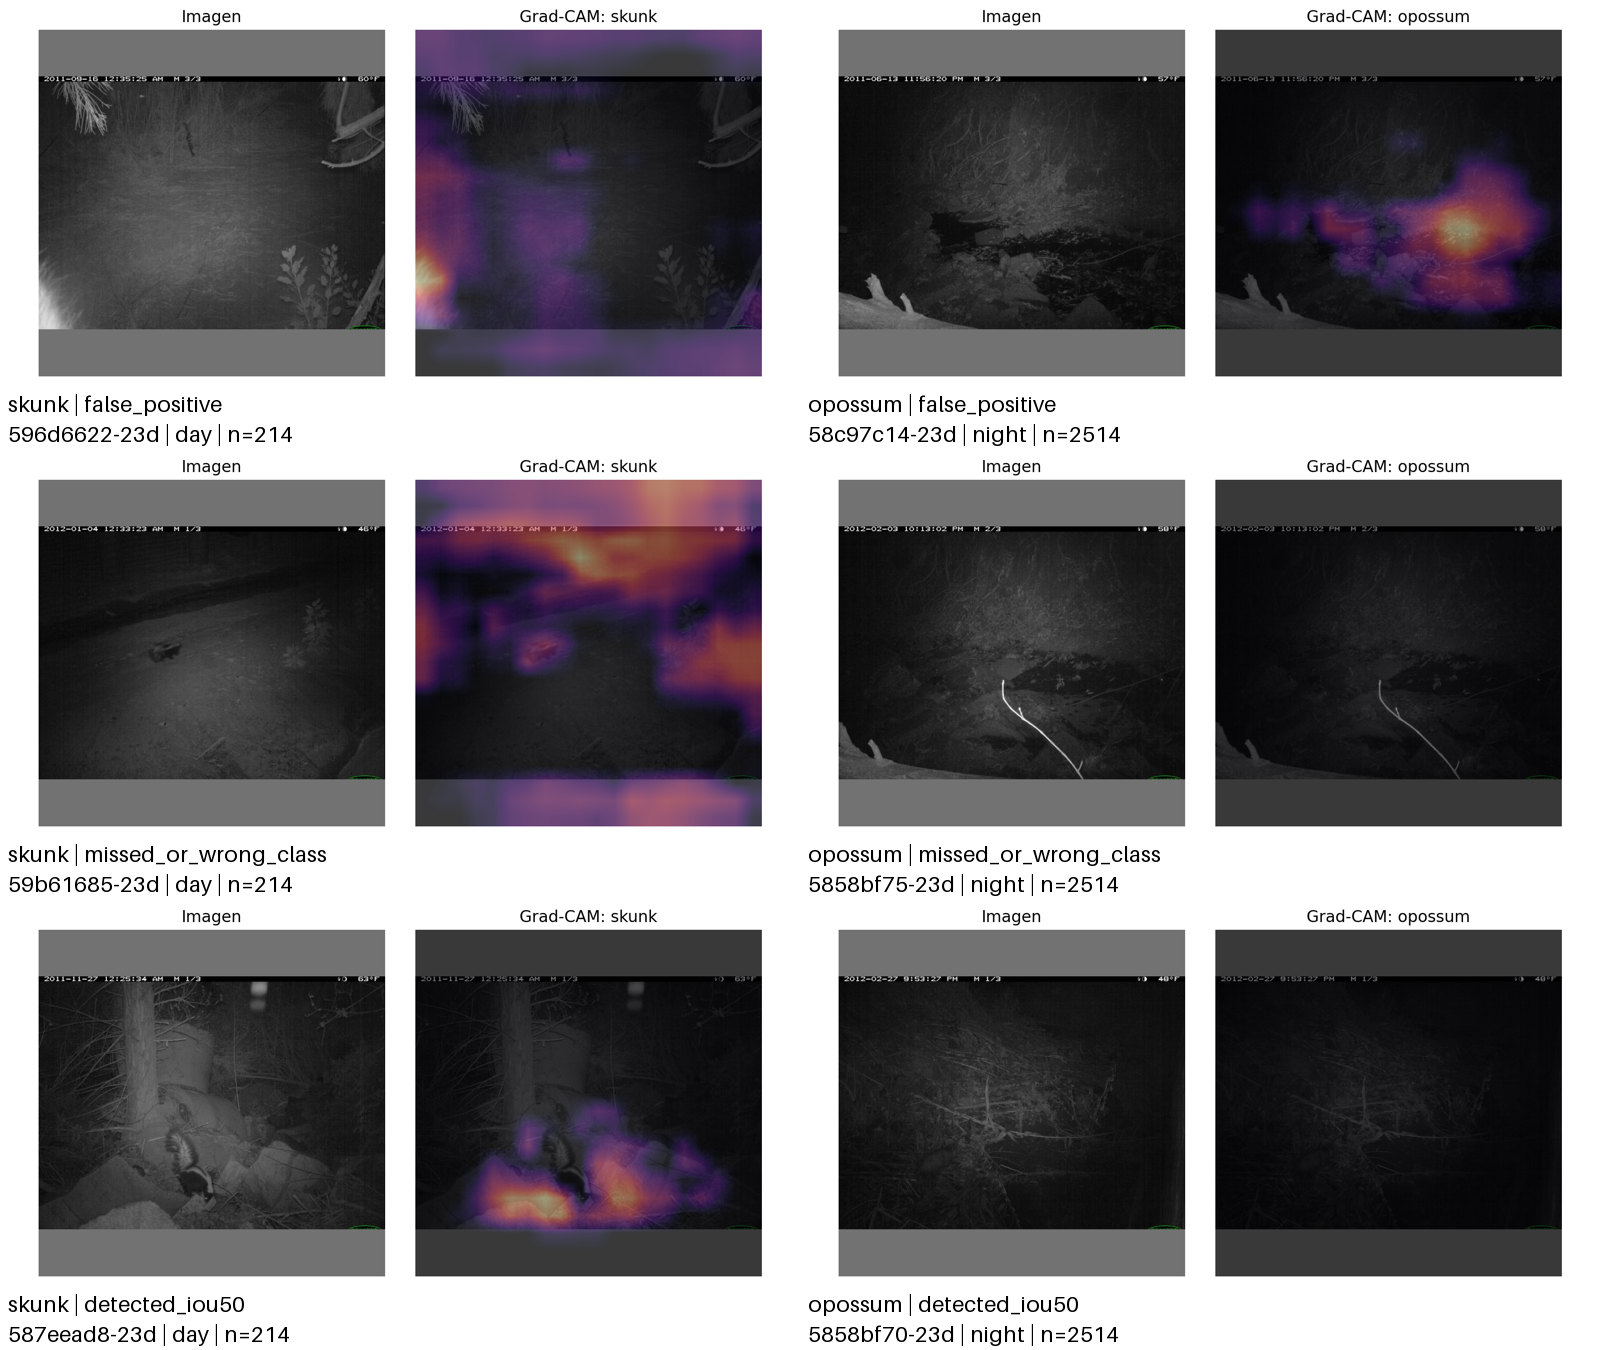
\includegraphics[width=\linewidth]{figures/figure_3.png}
\caption{Seis casos en cámaras nuevas. trans\_test\_3 y trans\_test\_5 tienen mapas planos. Las zonas resaltadas en fondos y bordes no demuestran causalidad ni memorización.}
\end{figure}
